 \documentclass[fleqn,11pt]{article}
\usepackage[letterpaper,margin=0.75in]{geometry}
\usepackage{amsmath}
\usepackage{booktabs}
\usepackage{graphicx}
\usepackage{listings}
\usepackage{caption}
\usepackage{tikz}
\usepackage{circuitikz}
\usepackage{enumerate}
\setlength{\parindent}{1.4em}

\begin{document}


\title{Coursework2}
\author{Yuli Zhi fh19804}
\date{}
\maketitle
\section*{PartA}
\subsection*{Question1}

\begin{center} 
    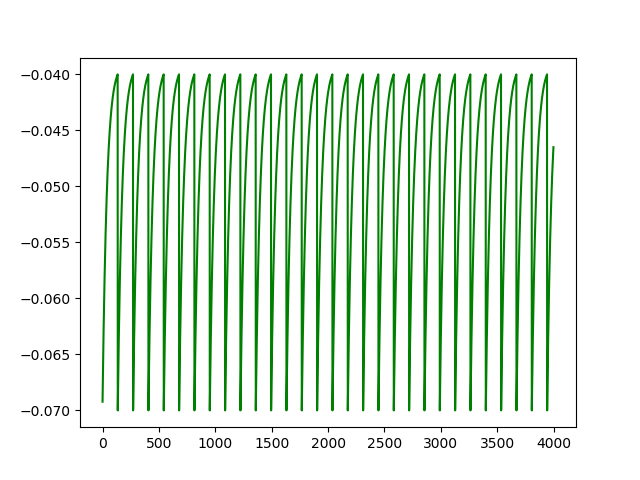
\includegraphics[width=10cm]{graphs/Question1.png}
    \captionof{figure}{Integrate Spike }
\end{center}

\subsection*{Question2}
\begin{center}
    \begin{minipage}{\linewidth} 
    \begin{minipage}{0.45\linewidth}
      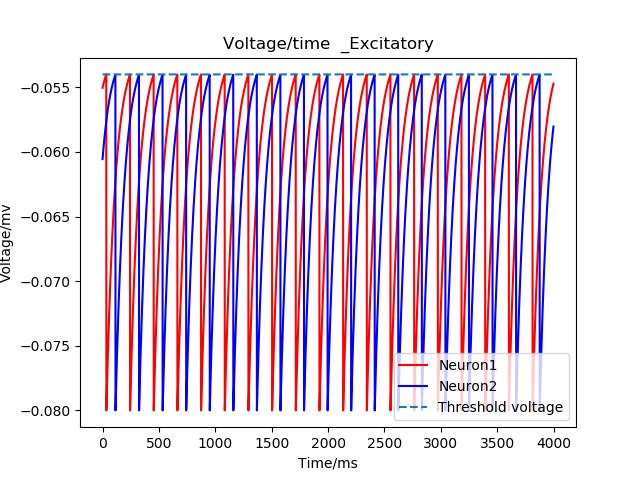
\includegraphics[width=7cm]{graphs/Question2_Excitatory.png}
      \captionof{figure}{Two neurons Excitatory} 
    \end{minipage}
    \hspace{0.05\linewidth}
    \begin{minipage}{0.45\linewidth}
      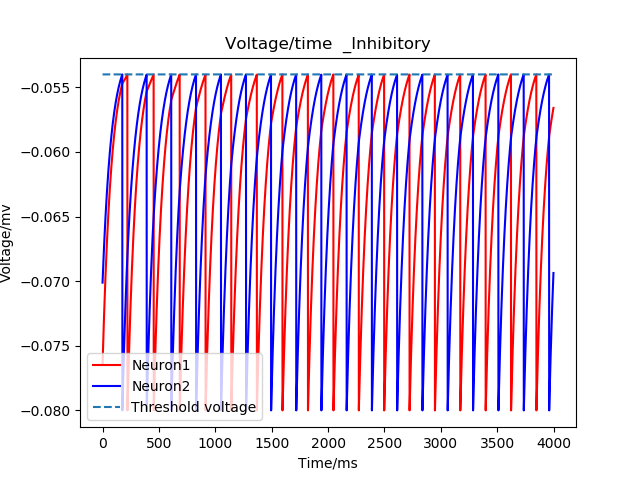
\includegraphics[width=7cm]{graphs/Question2_Inhibitory.png}
      \captionof{figure}{Two neurons Inhibitory}
    \end{minipage}
  \end{minipage} 
\end{center}
\par The left graph shows that two neurons have excitatory synaptic connections
    between each other, and the right is the inhibitory one. 
    Excitatory synaptic connection graph  shows that two neurons tend to synchronize.
    While in inhibitory connection, two neurons have different impulse times. 
    In the same time, One is impulse, and another is calm.                         
\newpage
\subsection*{COMSM2127}
\begin{enumerate}[1)]
\item  
  \par $I_e = (V_{th}-E_L)/R_m$
  \par the minimal current to produce an action potential  $I_e = 3nA$

\item
  \begin{center} 
    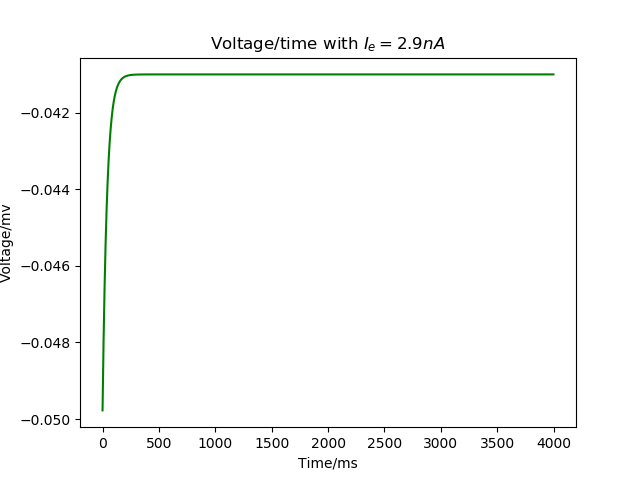
\includegraphics[width=10cm]{graphs/COMS2127_2.png}
    \captionof{figure}{Integrate Spike }
  \end{center}

\item
  \begin{center} 
    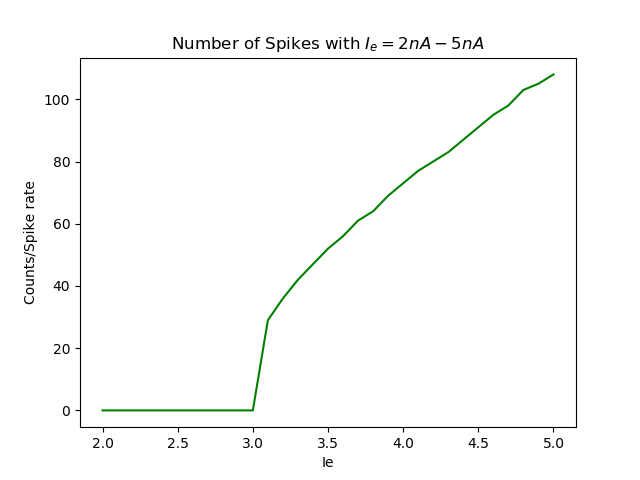
\includegraphics[width=10cm]{graphs/COMS2127_3.png}
    \captionof{figure}{Integrate Spike }
  \end{center}

\end{enumerate}

\newpage

\section*{PartB}
\end{document}



